\documentclass[border=10pt]{standalone}
\usepackage{pgfplots}
\pgfplotsset{compat=1.18}

\begin{document}
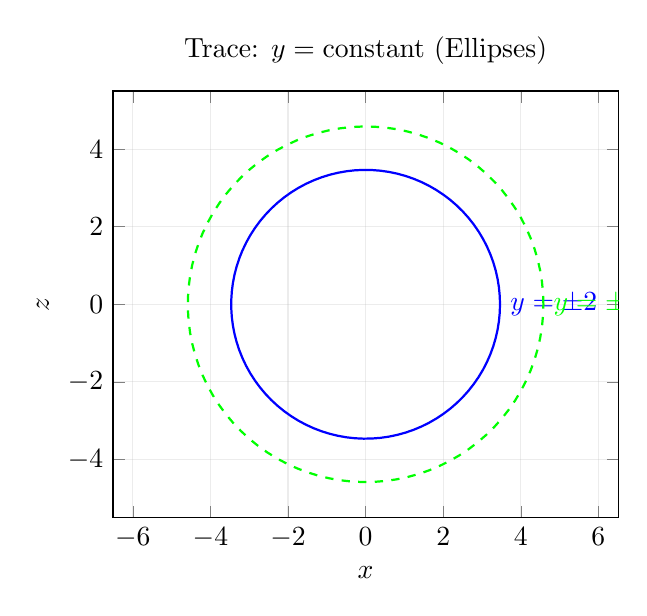
\begin{tikzpicture}
\begin{axis}[
    xlabel=$x$,
    ylabel=$z$,
    title={Trace: $y = \mathrm{constant}$ (Ellipses)},
    axis equal,
    grid=both,
    grid style={opacity=0.3},
    width=8cm,
    height=7cm,
    domain=0:360,
    samples=100,
]
% Ellipse for y = 2: x^2 + z^2 = 12
\addplot[blue, thick] ({sqrt(12)*cos(x)}, {sqrt(12)*sin(x)}) node[right] {$y = \pm 2$};
% Ellipse for y = 2.5: x^2 + z^2 = 21
\addplot[green, thick, dashed] ({sqrt(21)*cos(x)}, {sqrt(21)*sin(x)}) node[right] {$y = \pm 2.5$};
\end{axis}
\end{tikzpicture}

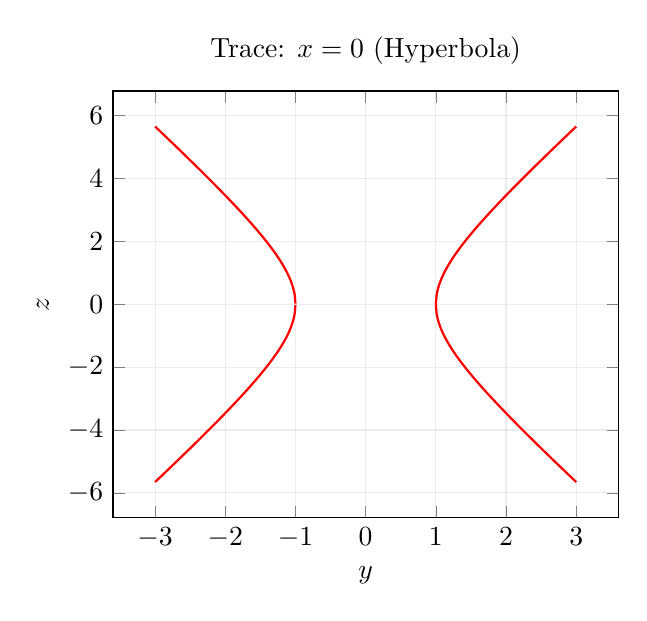
\begin{tikzpicture}
\begin{axis}[
    xlabel=$y$,
    ylabel=$z$,
    title={Trace: $x = 0$ (Hyperbola)},
    grid=both,
    grid style={opacity=0.3},
    width=8cm,
    height=7cm,
    domain=-3:3,
    samples=200,
]
% Hyperbola: 4y^2 - z^2 = 4 => z = \pm\sqrt{4y^2 - 4}
\addplot[red, thick, domain=-3:-1] {sqrt(4*x^2 - 4)};
\addplot[red, thick, domain=1:3] {sqrt(4*x^2 - 4)};
\addplot[red, thick, domain=-3:-1] {-sqrt(4*x^2 - 4)};
\addplot[red, thick, domain=1:3] {-sqrt(4*x^2 - 4)};
\end{axis}
\end{tikzpicture}

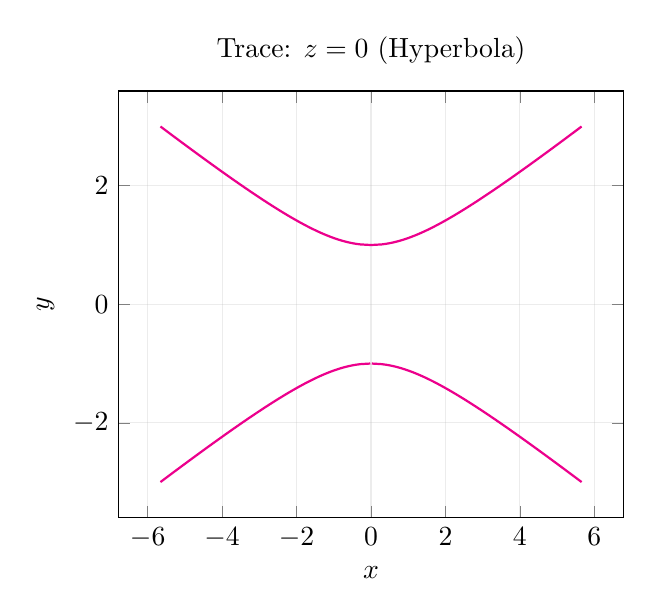
\begin{tikzpicture}
\begin{axis}[
    xlabel=$x$,
    ylabel=$y$,
    title={Trace: $z = 0$ (Hyperbola)},
    grid=both,
    grid style={opacity=0.3},
    width=8cm,
    height=7cm,
    domain=-5:5,
    samples=200,
]
% Hyperbola: -x^2 + 4y^2 = 4 => x = \pm\sqrt{4y^2 - 4}
\addplot[magenta, thick, domain=-3:-1] ({sqrt(4*x^2 - 4)}, {x});
\addplot[magenta, thick, domain=1:3] ({sqrt(4*x^2 - 4)}, {x});
\addplot[magenta, thick, domain=-3:-1] ({-sqrt(4*x^2 - 4)}, {x});
\addplot[magenta, thick, domain=1:3] ({-sqrt(4*x^2 - 4)}, {x});
\end{axis}
\end{tikzpicture}
\end{document}